% Options for packages loaded elsewhere
\PassOptionsToPackage{unicode}{hyperref}
\PassOptionsToPackage{hyphens}{url}
%
\documentclass[
  english,
  ,man,floatsintext]{apa6}
\usepackage{lmodern}
\usepackage{amssymb,amsmath}
\usepackage{ifxetex,ifluatex}
\ifnum 0\ifxetex 1\fi\ifluatex 1\fi=0 % if pdftex
  \usepackage[T1]{fontenc}
  \usepackage[utf8]{inputenc}
  \usepackage{textcomp} % provide euro and other symbols
\else % if luatex or xetex
  \usepackage{unicode-math}
  \defaultfontfeatures{Scale=MatchLowercase}
  \defaultfontfeatures[\rmfamily]{Ligatures=TeX,Scale=1}
\fi
% Use upquote if available, for straight quotes in verbatim environments
\IfFileExists{upquote.sty}{\usepackage{upquote}}{}
\IfFileExists{microtype.sty}{% use microtype if available
  \usepackage[]{microtype}
  \UseMicrotypeSet[protrusion]{basicmath} % disable protrusion for tt fonts
}{}
\makeatletter
\@ifundefined{KOMAClassName}{% if non-KOMA class
  \IfFileExists{parskip.sty}{%
    \usepackage{parskip}
  }{% else
    \setlength{\parindent}{0pt}
    \setlength{\parskip}{6pt plus 2pt minus 1pt}}
}{% if KOMA class
  \KOMAoptions{parskip=half}}
\makeatother
\usepackage{xcolor}
\IfFileExists{xurl.sty}{\usepackage{xurl}}{} % add URL line breaks if available
\IfFileExists{bookmark.sty}{\usepackage{bookmark}}{\usepackage{hyperref}}
\hypersetup{
  pdftitle={The Development of Color Terms in Shipibo-Konibo Children},
  pdfauthor={Danielle Kellier*1, Martin Fortier*2, Maria Fernández Flecha3, \& Michael C. Frank4},
  pdflang={en-EN},
  pdfkeywords={keywords},
  hidelinks,
  pdfcreator={LaTeX via pandoc}}
\urlstyle{same} % disable monospaced font for URLs
\usepackage{graphicx,grffile}
\makeatletter
\def\maxwidth{\ifdim\Gin@nat@width>\linewidth\linewidth\else\Gin@nat@width\fi}
\def\maxheight{\ifdim\Gin@nat@height>\textheight\textheight\else\Gin@nat@height\fi}
\makeatother
% Scale images if necessary, so that they will not overflow the page
% margins by default, and it is still possible to overwrite the defaults
% using explicit options in \includegraphics[width, height, ...]{}
\setkeys{Gin}{width=\maxwidth,height=\maxheight,keepaspectratio}
% Set default figure placement to htbp
\makeatletter
\def\fps@figure{htbp}
\makeatother
\setlength{\emergencystretch}{3em} % prevent overfull lines
\providecommand{\tightlist}{%
  \setlength{\itemsep}{0pt}\setlength{\parskip}{0pt}}
\setcounter{secnumdepth}{-\maxdimen} % remove section numbering
% Make \paragraph and \subparagraph free-standing
\ifx\paragraph\undefined\else
  \let\oldparagraph\paragraph
  \renewcommand{\paragraph}[1]{\oldparagraph{#1}\mbox{}}
\fi
\ifx\subparagraph\undefined\else
  \let\oldsubparagraph\subparagraph
  \renewcommand{\subparagraph}[1]{\oldsubparagraph{#1}\mbox{}}
\fi
% Manuscript styling
\usepackage{upgreek}
\captionsetup{font=singlespacing,justification=justified}

% Table formatting
\usepackage{longtable}
\usepackage{lscape}
% \usepackage[counterclockwise]{rotating}   % Landscape page setup for large tables
\usepackage{multirow}		% Table styling
\usepackage{tabularx}		% Control Column width
\usepackage[flushleft]{threeparttable}	% Allows for three part tables with a specified notes section
\usepackage{threeparttablex}            % Lets threeparttable work with longtable

% Create new environments so endfloat can handle them
% \newenvironment{ltable}
%   {\begin{landscape}\begin{center}\begin{threeparttable}}
%   {\end{threeparttable}\end{center}\end{landscape}}
\newenvironment{lltable}{\begin{landscape}\begin{center}\begin{ThreePartTable}}{\end{ThreePartTable}\end{center}\end{landscape}}

% Enables adjusting longtable caption width to table width
% Solution found at http://golatex.de/longtable-mit-caption-so-breit-wie-die-tabelle-t15767.html
\makeatletter
\newcommand\LastLTentrywidth{1em}
\newlength\longtablewidth
\setlength{\longtablewidth}{1in}
\newcommand{\getlongtablewidth}{\begingroup \ifcsname LT@\roman{LT@tables}\endcsname \global\longtablewidth=0pt \renewcommand{\LT@entry}[2]{\global\advance\longtablewidth by ##2\relax\gdef\LastLTentrywidth{##2}}\@nameuse{LT@\roman{LT@tables}} \fi \endgroup}

% \setlength{\parindent}{0.5in}
% \setlength{\parskip}{0pt plus 0pt minus 0pt}

% \usepackage{etoolbox}
\makeatletter
\patchcmd{\HyOrg@maketitle}
  {\section{\normalfont\normalsize\abstractname}}
  {\section*{\normalfont\normalsize\abstractname}}
  {}{\typeout{Failed to patch abstract.}}
\patchcmd{\HyOrg@maketitle}
  {\section{\protect\normalfont{\@title}}}
  {\section*{\protect\normalfont{\@title}}}
  {}{\typeout{Failed to patch title.}}
\makeatother
\shorttitle{Color Terms in Shipibo-Konibo Children}
\keywords{keywords\newline\indent Word count: X}
\usepackage{lineno}

\linenumbers
\usepackage{csquotes}
\ifxetex
  % Load polyglossia as late as possible: uses bidi with RTL langages (e.g. Hebrew, Arabic)
  \usepackage{polyglossia}
  \setmainlanguage[]{english}
\else
  \usepackage[shorthands=off,main=english]{babel}
\fi

\title{The Development of Color Terms in Shipibo-Konibo Children}
\author{Danielle Kellier*\textsuperscript{1}, Martin Fortier*\textsuperscript{2}, Maria Fernández Flecha\textsuperscript{3}, \& Michael C. Frank\textsuperscript{4}}
\date{}


\affiliation{\vspace{0.5cm}\textsuperscript{1} University of Pennsylvania\\\textsuperscript{2} PSL Research University\\\textsuperscript{3} Pontificia Universidad Católica del Perú\\\textsuperscript{4} Stanford University}

\abstract{
Enter abstract here. Each new line herein must be indented, like this line.
}



\begin{document}
\maketitle

TO BE PASTED FROM GOOGLE DOC

\hypertarget{introduction}{%
\section{Introduction}\label{introduction}}

Color language is where language and perception meet. Terms like \emph{blue} or \emph{red} draw boundary lines across a perceptually continuous space. In English, there are 11 basic color terms, but this color categorization is not universal. For instance, Russian speakers use two distinct words to describe the colors light blue (\enquote{goluboy}) and dark blue (\enquote{siniy}); and some languages have as few as two words (e.g., the Jalé people only have terms for ``light'' and ``dark''; Berlin \& Kay, 1969). Why do languages vary in their color systems? One emerging consensus is that languages categorize the color spectrum in different ways in part due to functional demands (Gibson et al., 2017): both smaller and larger color systems are relatively optimal for suiting different communicative needs (Regier, Kay, \& Khetarpal, 2007).
One important component of this hypothesis is the idea that some color systems are easier to learn for children than others; but the actual acquisition of color terms -- while well-studied in English (e.g., Wagner, Dobkins, \& Barner, 2013) -- is extremely under-studied across other populations. Berlin \& Kay's seminal World Color Survey (WCS; Kay, Berlin, Maffin, Merrifield, \& Cook, 2009) presented adult speakers of over 100 languages with differently colored chips and asked them to produce a label, characterizing the space of color vocabulary in a range of written and unwritten languages. The WCS is an invaluable resource for the cross-linguistic study of color vocabulary, but no comparable resource exists for cross-cultural studies of how this vocabulary is learned across childhood.
In the current project, our goals were (1) to characterize color term knowledge in an indigenous population previously studied by the WCS, the Shipibo-Konibo (SK), and then (2) to build on this foundation to characterize the developmental trajectory of color language acquisition in a group of children raised outside of the WEIRD (Western Educated Industrialized Rich Democratic) populations that are over-represented in behavioral science.

\hypertarget{color-in-amazonian-languages-and-latin-american-varieties-of-spanish}{%
\subsection{Color in Amazonian languages and Latin American varieties of Spanish}\label{color-in-amazonian-languages-and-latin-american-varieties-of-spanish}}

A few studies explore the use of color terms in the varieties of Spanish in Latin America. Berlin and Kay (1969) examine the case of the Mexican dialect of Spanish, which they consider to be in Stage VII of their classification. So, for example, a Stage II system would add the term red to the colors already present in Stage I (\emph{black} and \emph{white}). It wouldn't be possible for a system to have \emph{red} if it doesn't already have \emph{black} and \emph{white}. They identify the following basic color terms: \emph{blanco} (white), \emph{negro} (black), \emph{rojo} (red), \emph{verde} (green), \emph{amarillo} (yellow), \emph{azul} (blue), \emph{café} (brown), \emph{morado} (purple), \emph{rosa} (pink), \emph{anaranjado} (orange) and \emph{gris} (grey). Also, based on their work with forty Tzeltal participants, both Tzeltal monolinguals as well as Tzeltal-Spanish bilinguals, they found that bilingualism did not skew their results regarding the existence of semantic universals in the domain of color vocabulary. Tzeltal has five basic color terms: \emph{?ihk´} (black), \emph{sak} (white), \emph{cah} (red), \emph{yaš} (green) and \emph{k´an} (yellow). This language is estimated to be transitioning from Stage IV to V, which is reflected in the ambiguity of the focus of \emph{yaš} (grue). The authors posit that a long history of contact with Spanish has probably accentuated this, and suggest that exposure to Spanish in schools will eventually cause \emph{yaš} to be entirely restricted to greens, and \emph{azul} (or some other Spanish term) will be adopted into the Tzeltal color system.
Monroy and Custodio (1989) offers information on Colombian Spanish based on materials collected for the Linguistic-ethnographic Atlas of Colombia. He presents examples of ad hoc color terms referring to colors through objects prototypically instantiating these color: \enquote{vegetables}, \enquote{animals}, \enquote{food}, \enquote{metals}, \enquote{precious stones}, \enquote{fire and its derivatives} and \enquote{atmospheric phenomena}.
More recently, Aragón (2016) offers an ethnolinguistic study of color terms in Mexican Spanish: \emph{amarillo} (yellow), \emph{azul} (blue), \emph{blanco} (white), \emph{café} (literally \enquote{coffee}, but effectively brown), \emph{gris} (gray), \emph{morado} (purple), \emph{naranja} (orange), \emph{negro} (black), \emph{rojo} (red), \emph{rosado} (pink) and \emph{verde} (green). She analyzes the elaboration of these meanings in dictionaries, as well as the references and associations to which informants resort to for their own definitions. Aragón concludes that the local natural and cultural referents constitute a point of consensus among Mexicans when defining terms of color. Although informants also discussed some cultural material referents, these were not salient prototypes in their explanations. A special case that would merit further study in the future is that of \emph{café} in Mexico versus \emph{marrón} in Spain. According to the author, these two color terms are differentiated by the prototype \enquote{toasted coffee grain} associated to the Mexican Spanish term. Finally, she reviews the symbolic associations related to some terms, such as the discourses on femininity, especially those centered around the figure of the girl, associated with the term \emph{rosado.}
Gibson et al. (2017) offer some approximations to the case of color terms in Bolivian Spanish, based on their analysis centered on Tsimane, an indigenous language spoken by a group living in the Amazonian piedmont. The authors compare the Tsimane case with Bolivian Spanish and American English. Compared to Bolivian Spanish and English, Tsimane exhibits greater variability in terms of the color terms used for all color chips presented in their study, with the exception of red. Out of a total of 80 color chips, Tsimane exhibits 8 modal color terms while English has 10, and Bolivian Spanish, 11. Also, despite the variability observed, the assignment of modal color terms resulted in a similar partition of the color space in the three languages assessed. The authors also emphasize that the Tsimane color system is less informative than the English and the Bolivian Spanish one. Finally, using the free choice paradigm, they show speakers of Bolivian Spanish extensively use the term \emph{verde} (green) to denominate the color chips displayed, in addition to \emph{celeste} (light-blue) and \emph{azul} (blue), as well as \emph{morado} (purple). Less frequent terms are, for example, \emph{fucsia} (fuchsia), \emph{guinda} (maroon) and \emph{mostaza} (mustard).
Several indigenous Amazonian color systems have been studied in the WCS. One of them, Candoshi, has been further examined by Surrallés (2016). In this thought-provoking study, Surrallés suggests that no proper color term exists in this language. If the fieldworkers of the WCS found otherwise, it is only because they misidentified the elicited terms as color terms while they are nothing more than a series of ad hoc terms referring to objects or animals of the surrounding environment. For example, in Candoshi, the word for yellow is \enquote{\emph{ptsiyaromashi}} (\enquote{like the feathers of a milvago bird}), the word for red is \enquote{\emph{chobiapi}} (\enquote{ripe fruit}), the word for green is \enquote{\emph{kamachpa}} (\enquote{unripe fruit}), etc. These findings lead Surrallés to argue that the Candoshi do not have a proper color system. When they use \enquote{color terms} they are not trying to subsume objects of the world under abstract color categories, but they are rather establishing horizontal and ad hoc comparisons between similar objects of the world.
A similar criticism of the WCS approach had been previously developed by Everett (2005, pp. 627--628) based on his study of Pirahã, another Amazonian language. Everett also rejects the idea that there are basic color terms in this language. He argues that the four color terms identified as basic in the WCS are not such. For example, the word identified as the basic color term for \enquote{red} and \enquote{yellow} (\emph{bi i sai}) means nothing more than \enquote{bloodlike}. Here again, color terms seem to be ad hoc comparisons rather than proper basic terms.
As mentioned earlier, SK color terms have been thoroughly studied in the WCS. It is worth mentioning that two anthropological studies (Morin, 1973; Tournon, 2002) have also investigated the color terms used in this Amazonian language. However, these two studies contain some serious methodological pitfalls: a very limited number of chips were tested with only a few participants. As a result, we will not further discuss these studies in the remaining of this article and will only focus on a comparison with the WCS data.
In sum, while some dialectical differences can be noticed across varieties of Spanish, these slight variations are consistent with the general framework proposed by the WCS. Less consistent, however, is the recurrent finding that ad hoc terms seem to play a central role in Amazonian color systems -- and possibly also in some South-American varieties of Spanish (such as Colombian Spanish). More broadly, it seems that Amazonian color systems are characterized by fewer color terms than dialectical Spanish systems.

\hypertarget{the-development-of-color-vocabulary}{%
\subsection{The Development of Color Vocabulary}\label{the-development-of-color-vocabulary}}

\hypertarget{the-current-study}{%
\subsection{The Current Study}\label{the-current-study}}

In the last two decades, cross-cultural research aiming to go beyond North-American \enquote{convenience samples} has mainly focused on the study of East Asian children and adults. This endeavor has proved very fruitful (Kitayama \& Cohen, 2007) but is still limited because of its almost exclusive focus on North-American vs.~East-Asian samples. The current study contributes to the general effort to go beyond such samples and study the development of human cognition in a non-North American and non-East Asian context.
The SK people are an indigenous group located within the Peruvian Amazon. They are mainly horticulturalists, fishermen, occasionally hunters but are noted for their strong display of tradition despite increasingly regular interactions with the western world. Their children receive formal schooling for 4 hours a day and begin formal Spanish lessons closer to adolescence. Most SK adults have some grasp of Spanish but younger adults show more proficiency than elders.

The SK indigenous people are particularly interesting for at least two reasons:
They differ from samples usually studied by cross-cultural evolutionary psychologists (Apicella \& Barrett, 2016). Indeed, evolutionary psychologists are particularly interested in the study of contemporary hunter-gatherers because they are believed to be a good model of our Pleistocene ancestors. By contrast, like most riverine Amazonian cultures, the SK culture is not based on hunting and gathering, but on horticulture, fishing, and to a limited extent, hunting.
Because of their location on the Ucayali River, one of the main tributaries of the Amazon, the SK culture has always been enmeshed in rich trading networks involving other indigenous groups of the Andes and the Lowlands (in pre-conquest times) as well as Mestizos and Westerners (in post-conquest times) (Lathrap, 1970). It would thus be mistaken to think of this culture as an \enquote{isolated} or \enquote{preserved} one. On the contrary, having been extensively exposed to numerous cultural influences, the SK culture has been constantly reworked and reshaped through the centuries. This was especially true in the second half of the 20th century with intense contact with the Spanish-speaking Mestizo populations established along the Ucayali River. As a result, today's SK culture straddles two worlds.

\hypertarget{experiment-1}{%
\section{Experiment 1}\label{experiment-1}}

In our first experiment, our goal was to replicate and update the characterization of the adult SK color system given by the World Color Survey. We were further interested in the use of Spanish terms as language contact and multilingualism have increased in the years since the original World Color Survey work.

\hypertarget{methods}{%
\subsection{Methods}\label{methods}}

\hypertarget{participants}{%
\subsubsection{Participants}\label{participants}}

We recruited 39 adult participants (7 men). Most of participants were from SK communities of the Middle Ucayali region (from Yarinacocha, San Francisco, and Nueva Betania), but some of them were from communities of the Lower (Paoyhan) and Upper (Puerto Belen) Ucayali. In Yarinacocha (a small town located in the vicinity of Pucallpa), participants were recruited in Bena Jema, a neighborhood where most of the inhabitants are SK. All the other places where participants were recruited were native community villages exclusively inhabited by SK people. Overall, the sample included both somewhat urbanized SK (Yarinacocha and San Francisco) as well as SK individuals who were still used to more traditional activities and regular contact with the surrounding rainforest (Nueva Betania, Paoyhan, and Puerto Belen).

The median self-reported age for participants was 38 years with a range between 20 to 64 years of age (SD = 13.60yo). Regarding occupations, 41\% of the women were homemakers (33\% overall) and another 41\% were artisans (33\%). Three of the 7 men were horticulturalists (43\%, 8\% overall). Four women (12\%, 10\% overall) and three men (43\%, 8\% overall) identified as students.

Although all adult participants spoke Shipibo-Konibo as a first language, all were bilingual to a substantial degree. All reported an introduction to the Spanish language before early adolescence (\emph{M} = 7.80yo, \emph{SD} = 2.90y). Participant age and reported age of introduction to Spanish were positively correlated; younger participants reported learning Spanish at an early age although all participants reported introductions before early adolescence (\emph{r} = 0.43, \emph{p} = 0.01).

\hypertarget{materials}{%
\subsubsection{Materials}\label{materials}}

We used the 330 Munsell color chips as stimuli for the study. However, only 165 chips were used for each single participant (see below). These chips were exactly those used to collect data for the WCS. Individual color chips were 2 cm x 2.5 cm.

\hypertarget{procedure}{%
\subsubsection{Procedure}\label{procedure}}

In order to make sure that the natural light intensity would not vary much between participants, the experiment took place indoors, near a window or a door. The study was conducted entirely in the SK language.

Our procedure was similar to that used in the WCS (see Kay et al., 2009, pp. 585--591). Participants were seated in front of the experimenter and introduced to the whole procedure and the general goal of the study. Then the primary procedure involved presenting participants with a color chip and asking them: \enquote{What is the color of this chip?}\footnote{The SK word for color that we used was the Spanish word \emph{color}. In general, the SK language includes some castillanisms that are well-known by all speakers; color is one of them.} and recording their response or responses.

One major difference between the WCS procedure and ours is that, in the WCS, the experimenter was expected to brief participants so that they would only provide basic color terms during the task (e.g., \enquote{blue} as opposed to \enquote{navy blue} or \enquote{sky-like}). However, we found it rather difficult to help participants understand in a few sentences what a basic color term was.\footnote{Indeed, as Berlin \& Kay (2009: 587-589) acknowledge, there is no straightforward necessary and sufficient criteria for the \enquote{basicness} of a color term.} Thus, we opted to let participants provide any term they wished. If they did not provide a basic color term, we would ask further questions to elicit a basic color term. For example, if the participant provided the term \enquote{blood-like} (a non-basic color term) when presented with a red color chip, the experimenter would ask: \enquote{Do you know of any other word to refer to the color of this chip?} If the participant subsequently responded \enquote{dark red} (another non-basic color term), the experimenter would further ask: \enquote{How would you refer to this color with only one word?} Eventually, the participant would say \enquote{red} (a basic color term).

For some chips, participants would provide a basic color term at once; but for others, they would first provide one or two non-basic terms before actually providing a basic term. When participants did not provide a basic color term after three trials (i.e., two follow-up questions), no further questions was asked, and the experimenter proceeded to the next chip. This method was more effortful and time-consuming than the WCS procedure, but it improved the fluency and the intuitiveness of the task for participants.

A second difference between our procedure and that of the WCS concerned the number of chips each participant was presented with. In the WCS, every participant was expected to provide color terms for each of the 330 chips of the set. As we were afraid that doing so would take too long and that participants would find the task tedious, we decided that the set of chips would be split in two (even and uneven numbers) and that every participant would be randomly ascribed to one of the two subsets. As a result, each participant was presented with only 165 chips.

\hypertarget{results-and-discussion}{%
\subsection{Results and Discussion}\label{results-and-discussion}}

\begin{figure}
\centering
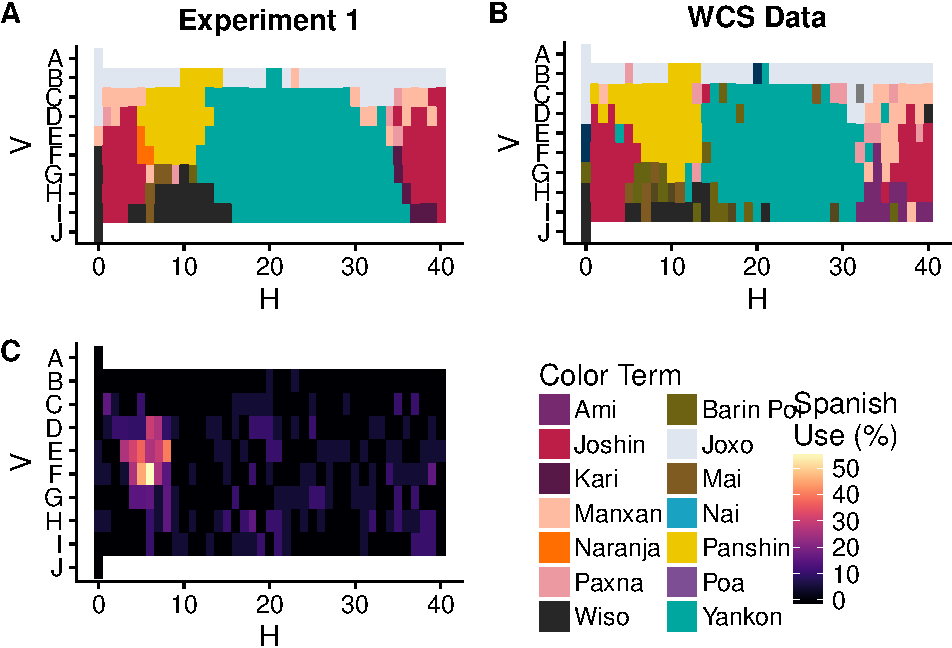
\includegraphics{amazon_color_files/figure-latex/adultfigure-1.pdf}
\caption{\label{fig:adultfigure}(A and B) Plots of the modal term given for a particular chip. Color coordinates were represented in 2-D Munsell space. Modal responses were given by SK adults during (A) the original World Color Survey and during (B) our Experiment 1. (C) Heat map of prevalence of Spanish-language responses during Experiment 1. Legends for all three subplots located in the bottom-right quadrant.}
\end{figure}

Broadly speaking, our results were quite similar to the WCS findings. Figure 1 shows a comparison between our data (Panel A) and the WCS (panel B). The basic level colors in our data were quite similar, as well. All participants described at least 1 chip with the following set of color terms: light/white (\enquote{joxo}), dark/black (\enquote{wiso}), yellow (\enquote{panshin}), red (\enquote{joshin}), and green/blue (\enquote{yankon}). Most (79\%) participants also used described at least 1 chip as faded or \enquote{manxan}, referring to a chip's saturation. In terms of overall popularity, participants on average described 32\% of chips as \enquote{yankon} (\emph{SD} = 10\%) followed by \enquote{joshin} (\emph{M} = 12\%, \emph{SD} = 6\%), \enquote{joxo} (10\%, 5\%), \enquote{panshin} (9\%, 4\%), \enquote{manxan} (7\%, 7\%), and \enquote{wiso} (6\%, 4\%).

One departure from the Berlin-Kay data was that 59\% of adults described at least 1 chip using a Spanish-language color term, accounting for 4\% of all responses (Figure 1, Panel C). In particular, Spanish use reached as high as 55\% when participants were asked to label chips that English speakers would consider to be orange, or \enquote{naranja} in Spanish. However, there was a high amount of variability in Spanish use between subjects (\emph{M} = 4\%, \emph{SD} = 12\%) which neither participant age (\emph{p} = 0.87) nor reported age of Spanish introduction (\emph{p} = 0.56) failed to predict. Some subjects never responded in Spanish whereas one participant used Spanish labels for 71\% of all trials despite all sessions being conducted entirely in the Shipibo-Konibo language. While we can only speculate as to this participant's motivations, it seems likely that they were more familiar with Spanish color vocabulary or viewed Spanish color terms as more precise descriptors.

Participants on average described 69\% of chips using a SK basic color term like \enquote{yankon} (\emph{SD} = 22\%). Some participants described chips using SK ad-hoc color terms, such as \enquote{nai} or \emph{sky} for blue chips (\emph{M} = 11\%, \emph{SD} = 12\%), or ad hoc terms referring to saturation or luminosity of a chip, such as \enquote{manxan} (\emph{M} = 7\%, \emph{SD} = 7\%). Virtually all instances where a participant responded in Spanish involved a Spanish basic color term such as \enquote{rojo} (\emph{M} = 4\%, \emph{SD} = 10\%). In other words, participants typically only responded in Spanish to label chips into basic categories; they relied on Shipibo-Konibo for other descriptors.

Given these data, we moved on to exploring the development of SK color vocabulary in childhood. Experiment 2 tests production and comprehension of SK color terms using SK-prototypical color chips; Experiment 3 tests children in Spanish using Spanish-prototypical chips.

\hypertarget{experiment-2}{%
\section{Experiment 2}\label{experiment-2}}

In Experiment 2, we tested children on their production and comprehension skills with a set of chips representing the prototypical colors for common SK color terms.

\hypertarget{methods-1}{%
\subsection{Methods}\label{methods-1}}

\hypertarget{participants-1}{%
\subsubsection{Participants}\label{participants-1}}

\begin{table}[tbp]
\begin{center}
\begin{threeparttable}
\caption{\label{tab:unnamed-chunk-2}Demographics of participants in Experiment 2.}
\begin{tabular}{lll}
\toprule
Age Group & \multicolumn{1}{c}{N} & \multicolumn{1}{c}{Male}\\
\midrule
5 & 3 (5\%) & 1 (33\%)\\
6 & 8 (14\%) & 3 (38\%)\\
7 & 12 (21\%) & 4 (33\%)\\
8 & 15 (26\%) & 5 (33\%)\\
9 & 10 (18\%) & 5 (50\%)\\
10 & 4 (7\%) & 2 (50\%)\\
11 & 5 (9\%) & 3 (60\%)\\
\bottomrule
\end{tabular}
\end{threeparttable}
\end{center}
\end{table}

The Pontificia Universidad Católica del Perú's Institutional Review Board approved our study protocol. We recruited 57 5- to 11-year-old children (23 boys). Table 1 shows the distribution of ages and genders. Fifteen children were recruited from neighborhoods in Yarinacocha, in the Pucallpa region of Peru, as well as in 42 children from Bawanisho, a native community settled along the Ucayali River, south of Pucallpa. Children were recruited either through their parents or through local schools. When recruited at school, consent for participation was collected from both the teachers and the parents; otherwise, only consent from the parents was collected.

\hypertarget{materials-1}{%
\subsubsection{Materials}\label{materials-1}}

Based on findings of Experiment 1, we selected out 8 color chips that were prototypical instances of prominent SK color terms. These color chips were blue (WCS n°1), green (WCS n°234), red (WCS n°245), white (WCS n°274), yellow (WCS n°297), black (WCS n°312), greeny-yellow (WCS n°320), and purple (WCS n°325). These color chips were exactly the same as those used in Experiment 1; the only difference was that adult participants in Experiment 1 were presented with these chips along the rest of their assigned 165 chip set. Child participants only had these 8 chips.

\hypertarget{procedure-1}{%
\subsubsection{Procedure}\label{procedure-1}}

The production and comprehension tasks were both conducted in SK. In both tasks, children were seated in front of the experimenter. A table on which the color chips were display stood between them. The production task was always performed before the comprehension task.

\textbf{Production task.} The procedure was very similar to that of Experiment 1. Children were first introduced to the whole procedure and the general goal of the study. It was specified that they would be expected to provide color terms in SK (and not in Spanish). Children were then asked: \enquote{What is the color of this chip?}. As with adults, we used follow-up questions to elicit basic color terms when the terms children initially provided were not basic. When children provided Spanish color terms, the experimenter would write down their response but further ask: \enquote{What is the name of this color in SK?} When children replied \enquote{I don't know} to this prompt, the experimenter would not ask further questions and would move forward to the next color chip. As a result, responses of some children include only non-basic SK color terms or Spanish color terms. In total, we collected production data for 8 color chips. For each chip, the data include either one response (when children provided a SK basic color term in the first trial) or two or three responses (when children's initial responses were either non-basic and/or in Spanish).

Further, Experiment 1 showed that for some of these color terms, only one response was accurate, while for others, several responses were equally correct. For example, responses during Experiment 1 to a particular purple chip ranged from red to blue with some using the terms ami (\enquote{flower}) or pua (\enquote{yam}) as common descriptors. Accuracy was coded based on the results derived from Experiment 1: if at least 15\% of participants in Experiment 1 labeled a chip with a particular term, we considered a trial to be correct if the child made the same pairing, regardless of whether the term as a basic or ad-hoc color term.

\textbf{Comprehension task.} The 8 color chips of the production task were simultaneously displayed in front of the children. The experimenter would then ask: \enquote{Can you give me the {[}color{]} chip?} In total, the comprehension of 9 SK color terms was tested. The choice of these terms was based on the findings of Experiment 1. Not all of them were basic, but all of them stood out as being prominent in the SK color system. The 9 terms used as prompts included: yankon (\enquote{green/blue}), joshin (\enquote{red}), panshin (\enquote{yellow}), joxo (\enquote{white), wiso (}black\enquote{), nai (}blue\enquote{), and barin poi (}greeny-yellow\enquote{). In addition, as Experiment 1 revealed that two non-basic terms are widely used to refer to green and purple, two words were used to test comprehension of each of these two colors: pei/xo (}green\enquote{) and ami/pua (}purple").

When the experimenter asked children to pick up a color that was instantiated by several chips, we followed the following procedure. The experimenter would ask: \enquote{Can you give me the {[}color{]} chip?} Children would then pick up a chip. The response would be registered and the chip be taken out of the table. As a result, only 7 chips would be remaining on the table. The experimenter would subsequently ask: \enquote{Can you give me another {[}color{]} chip?}. Children would then pick up a new chip. The response would be registered and the chip be taken out of the table. The experimenter would then ask the same question again until a total of as many times as there were correct instances. Thus, for \enquote{yankon}, four chips would be elicited, whereas for \enquote{joshin} or \enquote{pei/xo}, two chips would be elicited. Like the preceding production task, accuracy was scored based on responses given in Experiment 1. Similar to the production task, a child's choice for a particular chip was deemed accurate if at least 15\% of Experiment 1 participants made the same chip-label association. Unlike the production task, as some trials could have multiple pairings, accuracy was scored as an average, rather than dichotomous. For instance, if a child correctly chose 3 out of 4 chips for the \enquote{yankon} trial, they received a score of 0.75.

\hypertarget{results-and-discussion-1}{%
\subsection{Results and Discussion}\label{results-and-discussion-1}}

\begin{figure}
\centering
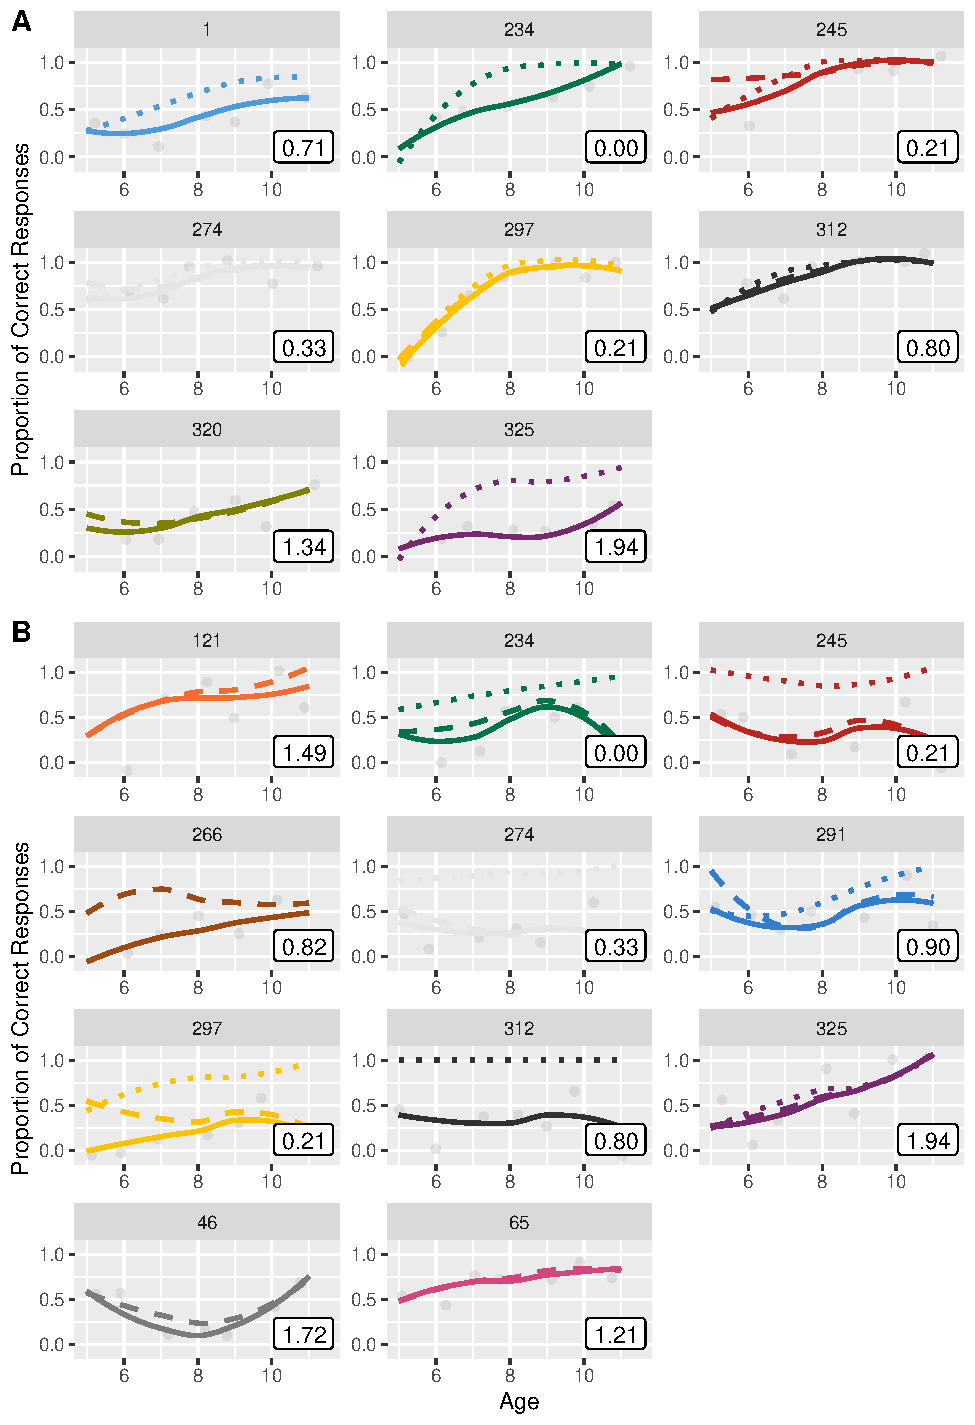
\includegraphics{amazon_color_files/figure-latex/prod_childfigure-1.pdf}
\caption{(\#fig:prod\_childfigure)(A and B) A comparison of children's performance during the production task in Studies 2 (top) and 3 (bottom). Solid or dotted lines represent overall performance by age for a particular chip. Solid lines show whether the child gave a correct answer in the language indicated in that column; dotted lines show if they gave a response that was correct in either language. Line colors are representative of the chip's color coordinates.}
\end{figure}

\hypertarget{production}{%
\subsubsection{Production}\label{production}}

Children's production accuracy increased substantially across nearly all color chips in the age range that we tested. Figure 2, top panel shows the accuracy of children's first production, both in SK (solid line) and in either language (dashed line). To quantify these developmental trends, we fit two generalized linear mixed effects models, one for the accuracy of SK production and one for the accuracy of production in either language. Both of these predicted accuracy as a function of the child's age, and included random intercepts for color chip and for participant, as well as a random slope of age by color chip. Age was a significant predictor in both models: \(\beta = 1.05\), SE = 0.28, \(p = 0.00\) and \(\beta = 1.11\), SE = 0.23, \(p < .0001\).

Over a quarter (28\%) of all responses were given in Spanish, and the distribution of Spanish responses was non-random. Children tended to respond in Spanish when presented with a chip with low naming consensus among adult participants in Experiment. As an exploratory analysis, we attempted to quantify low naming consensus using naming entropy (following Gibson et al., 2017). We computed the naming entropy for each chip by computing the probabilities for each chip \(c\) to be named with a particular label \(l\) (\(p(l \mid c)\)) and then taking \(H(c) = - \sum{p(l\mid c) \log[p(l \mid c)]}\) (see inset entropy values by chip in Figure 2).

To assess the hypothesis that naming entropy in adults was related to Spanish use in children, we fit a mixed effects model predicting Spanish responses as a function of age, entropy of the chip's naming distribution for adults, and their interaction. We included random intercepts for color chip and for participant, but our model did not converge with a random slope term and so we pruned this term following our lab's standard operating procedure. We found a reliable effect of entropy (\(\beta = -6.09\), SE = 2.38, \(p = 0.01\)) and an interaction between age and entropy (\(\beta = -3.97\), SE = 1.49, \(p = 0.01\)), suggesting that adults' uncertainty regarding naming was related to children's likelihood of producing Spanish labels.

One reason to use Spanish would be if children fail to recall the proper SK color term but do know the proper mapping in the Spanish. But another possibilitiy is that children may have more imprecise representations and choose to respond with a same-language but adjacent color term (such as \enquote{joshin} for a \emph{panshin}-colored chip). In our next analysis, following Wagner et al. (2013), we aggregate across color chips and examine the pattern of children's first responses, categorizing them as same-language, adjacent, and different-language. This analysis is shown in Figure 3, left panel.

We fit a mixed-effects model predicting correct performance with predictors specified as above, but including only random intercepts for participants due to convergence issues). We found a significant improvement in accuracy scores when we allowed different-language but corresponding responses (\emph{p} \textless{} 0.001) but no significant change when allowing for same-language but adjacent responses (\emph{p} = 0.409). This result suggests that children's incorrect responding was not due to imprecise knowledge of SK terms.

\begin{figure}
\centering
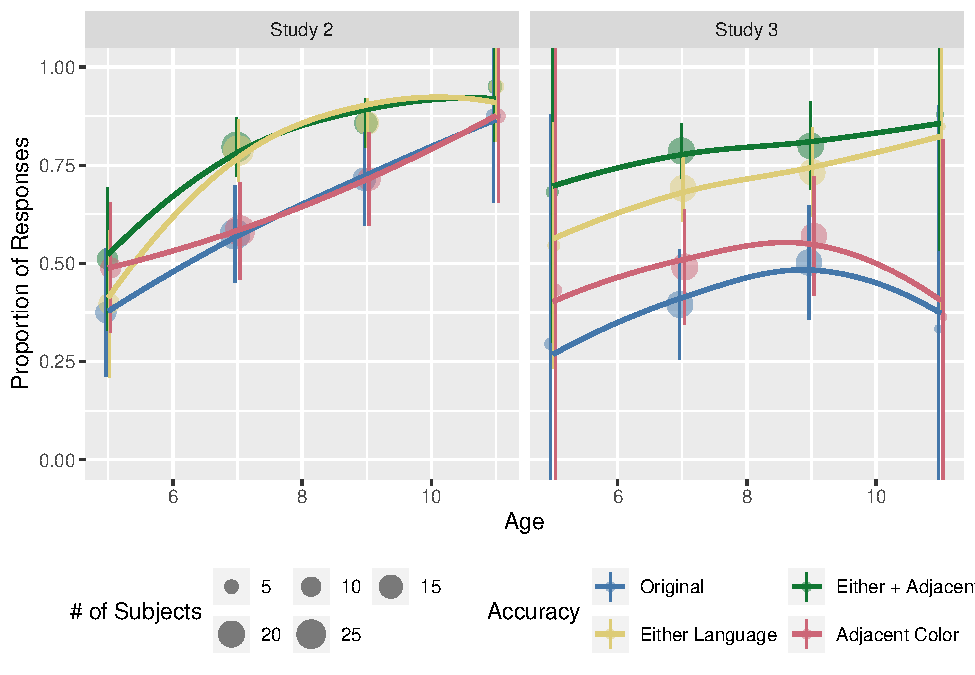
\includegraphics{amazon_color_files/figure-latex/study23accuracyplots_prod-1.pdf}
\caption{(\#fig:study23accuracyplots\_prod)Proportion of accurate responses when applying different accuracy criteria, by age and experiment. Points show the mean for a 2-year age group (chosen arbitrarily for visualization) with 95\% confidence intervals. Lines show a loess smoothing function.}
\end{figure}

\hypertarget{comprehension}{%
\subsubsection{Comprehension}\label{comprehension}}

\begin{figure}
\centering
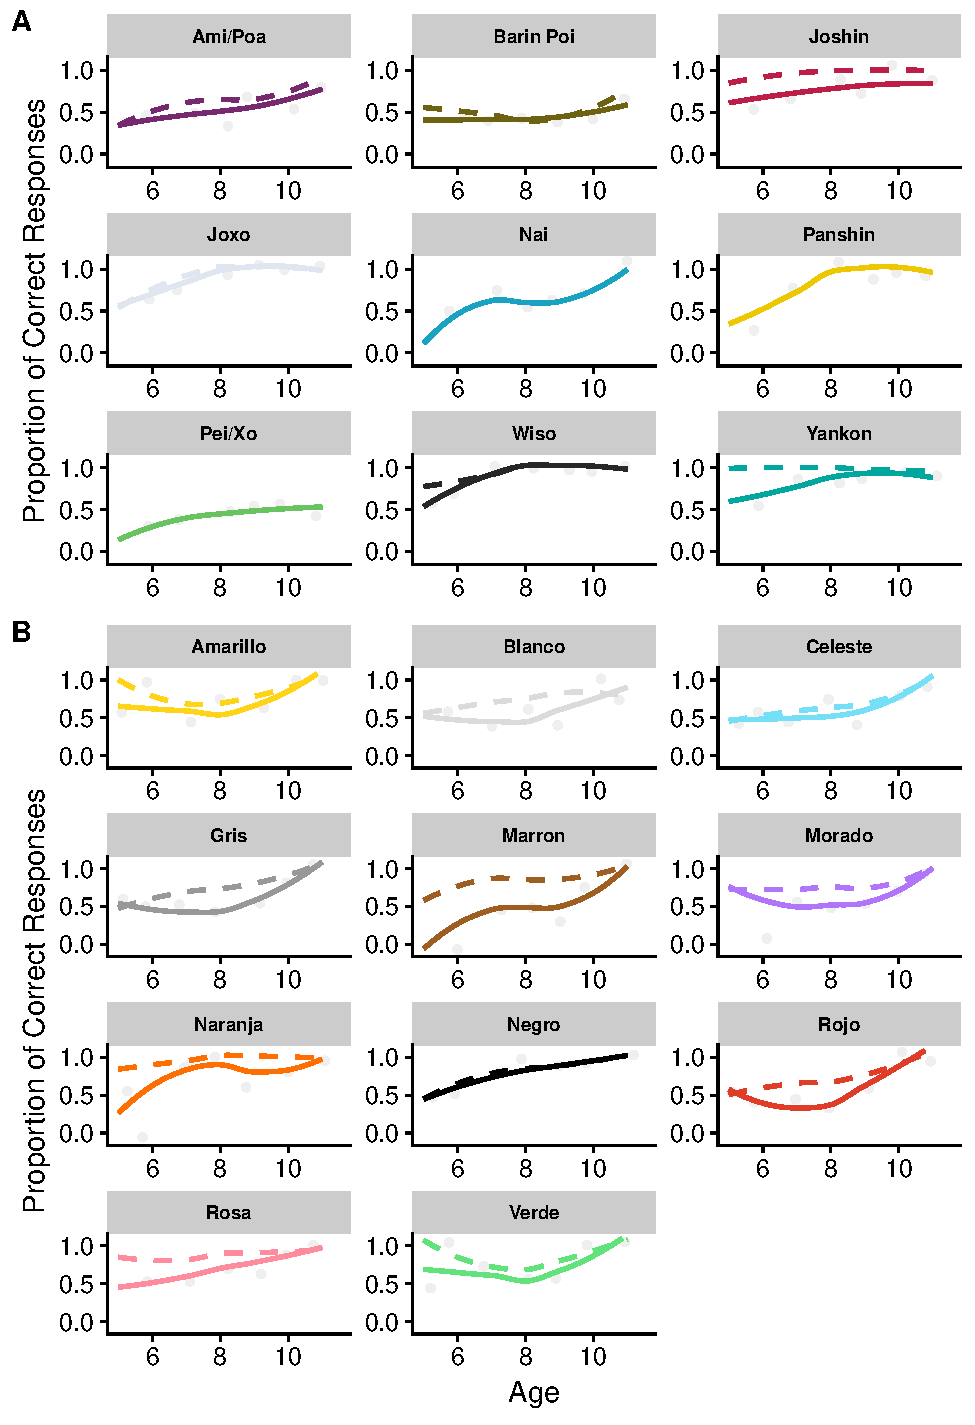
\includegraphics{amazon_color_files/figure-latex/comp_childfigure-1.pdf}
\caption{(\#fig:comp\_childfigure)(A and B) A comparison of children's performance during the comprehension tasks in Studies 2 (top) and 3 (bottom). Solid or dotted lines represent overall performance by age for a particular chip. Solid lines show whether the child chose the correct chip when prompted with a color term; dotted lines show whether a child chose the correct chip or a chip from an adjacent color category. Line colors are representative of the label's prototypical color coordinates.}
\end{figure}

Children's accuracy in the comprehension task increased with age across nearly all color chips. Figure 4, panel A shows the accuracy of children's comprehension, both for strict accuracy (solid line) and lenient accuracy---allowing chips for adjacent colors (dashed line). Like the production task, we fit two generalized linear mixed effects models, one for strict scoring of SK comprehension and another for lenient scoring of accurate or adjacent chips. Both of these predicted accuracy as a function of the child's age, and included random intercepts for color chip and for participant, as well as a random slope of age by color chip. Age was a significant predictor in both models: \(\beta = 0.60\), SE = 0.18, \(p = 0.00\) and \(\beta = 0.67\), SE = 0.19, \(p < .0001\).
Comparing strict accuracy across both production and comprehension tasks for Experiment 2, there is a stronger developmental trajectory seen in the production task. This pattern holds true even when allowing for responses involving adjacent color categories. The smaller intercept and beta weight for comprehension task with both strict and lenient scoring may shed some light on children's failure to recall during the earlier production task. During the production task, children may decide to use a Spanish color term if they fail to recall the proper SK term, however they were less likely to use the SK term for an adjacent color category. In addition, their performance did not improve when they were provided with a label and asked to map it to a limited set of chips. If SK children developed their color-term mapping by originally overextending categories and slowly refining their boundaries, we would have seen a marked improvement in performance once we scored for adjacent categories. In addition, if SK children were aware of the color category but merely failed to recall its corresponding term, children should have performed better in the later comprehension task upon being prompted with the missing label. However, we failed to find evidence that SK children's development of categorical boundaries well preceeded acquisition of SK terms.

\begin{figure}
\centering
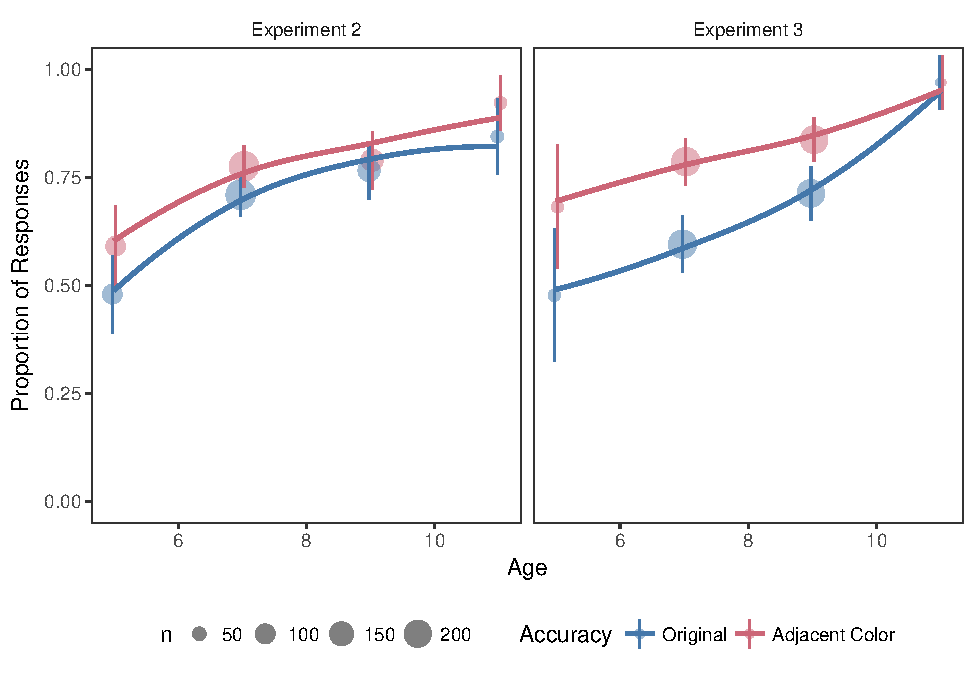
\includegraphics{amazon_color_files/figure-latex/study23accuracyplots_comp-1.pdf}
\caption{(\#fig:study23accuracyplots\_comp)Proportion of accurate responses when applying different accuracy criteria, by age and experiment. Points show the mean for a 2-year age group (chosen arbitrarily for visualization) with 95\% confidence intervals. Lines show a loess smoothing function.}
\end{figure}

\hypertarget{experiment-3}{%
\section{Experiment 3}\label{experiment-3}}

Noting the level of bilingualism in the SK population, we designed Experient 3 as its complement. Due to the length of these experiments, however, as well as the task demands involved in testing the same children sequentially in both languages, we chose to perform this next experiment with a separate group of children. In Experiment 3, we tested children entirely in Spanish with a set of chips representing prototypical colors for the Spanish color system.

\hypertarget{participants-2}{%
\subsubsection{Participants}\label{participants-2}}

\begin{table}[tbp]
\begin{center}
\begin{threeparttable}
\caption{\label{tab:unnamed-chunk-5}Demographics of participants in Experiment 3.}
\begin{tabular}{lll}
\toprule
Age Group & \multicolumn{1}{c}{N} & \multicolumn{1}{c}{Male}\\
\midrule
5-years-old & 2 (4\%) & 1 (50\%)\\
6-years-old & 2 (4\%) & 0 (0\%)\\
7-years-old & 11 (24\%) & 4 (36\%)\\
8-years-old & 9 (20\%) & 1 (11\%)\\
9-years-old & 11 (24\%) & 4 (36\%)\\
10-years-old & 8 (17\%) & 3 (38\%)\\
11-years-old & 3 (7\%) & 3 (100\%)\\
\bottomrule
\end{tabular}
\end{threeparttable}
\end{center}
\end{table}

As with Experiment 2, our protocol received ethical approval from Pontificia Universidad Católica del Perú's Institutional Review Board. Children were recruited in a SK neighborhood of Yarinacocha (Bena Jema) as well as in Bawanisho. As before, children were recruited either through their parents or through the local school. When recruited at school, consent for participation was collected from both the teachers and the parents; otherwise, only consent from the parents was collected. Data were collected from a total of 46 children (16 boys) between the ages of 5 and 11 years old.

\hypertarget{materials-2}{%
\subsubsection{Materials}\label{materials-2}}

Even though participants in Experiment 3 were instructed to give color terms in SK, some Spanish color terms were provided (this was especially true of younger adult participants, who were more proficient in Spanish). Based on these data and on previous studies of Spanish color systems, we singled out 11 color chips that were prototypical instances of prominent Peruvian Spanish color terms. These color chips were grey (WCS n°46), pink (WCS n°65), orange (WCS n°121), green (WCS n°234), red (WCS n°245), brown (WCS n°266), white (WCS n°274), blue (WCS n°291), yellow (WCS n°297), black (WCS n°312) and purple (WCS n°325). These color chips were exactly the same as those used in Experiment 1; the only difference was that while 330 chips were used in Experiment 1, only 11 of them were used in Experiment 3. Six chips were shared between Experiment 2 and Experiment 3.

\hypertarget{procedure-2}{%
\subsubsection{Procedure}\label{procedure-2}}

Since SK children are not very fluent in Spanish, the production and comprehension tasks were both conducted in SK, and Spanish was only used for color terms (i.e., Spanish color terms were embedded in SK sentences). As in Experiment 2, the production task was always performed before the comprehension task.

\textbf{Production task.} The procedure was the same as that of Experiment 2. Children were first introduced to the whole procedure and the general goal of the study. It was specified that they would be expected to provide color terms in Spanish (and not in SK). Children were then asked: \enquote{what is the color of this chip?} When children provided SK color terms, the experimenter would write down their response but further ask: \enquote{what is the name of this color in Spanish?} When children replied \enquote{I don't know} to this prompt, the experimenter would not ask further questions and would move forward to the next color chip. As a result, responses by some children include only non-basic Spanish color terms or SK color terms. For each chip, the data include either one response (when children provided a Spanish basic color term in the first trial) or two or three responses (when children's initial responses were either non-basic and/or in SK).

\textbf{Comprehension task.} The procedure was identical to that of the comprehension task of Experiment 2, with the exception of the set of chips and labels. In total, the comprehension of 11 Spanish color terms was tested. The choice of these terms was based on previous studies examining Spanish color terms as well as on Experiment 1. The 11 terms used as prompts included: blanco (\enquote{white}), verde (\enquote{green}), rojo (\enquote{red}), amarillo (\enquote{yellow}), azul (\enquote{blue}), negro (\enquote{black}), naranja (\enquote{orange}), gris (\enquote{grey}), morado (\enquote{purple}), marrón (\enquote{brown}), and rosa (\enquote{pink}). Since each color term was instantiated by only one color chip, no term required the special procedure that was followed in Experiment 2 for the ambiguous terms.

\hypertarget{results-and-discussion-2}{%
\subsection{Results and Discussion}\label{results-and-discussion-2}}

\hypertarget{production-1}{%
\subsubsection{Production}\label{production-1}}

The results of the production task are shown in Figure 2, bottom panel. Qualitatively, we saw smaller developmental effects. As in Experiment 2, we fit two generalized linear mixed effects models, one for the accuracy of Spanish term production and one for the accuracy of production in either language. Both of these predicted accuracy as a function of the child's age, and included random intercepts for color chip and for participant, as well as a random slope of age by color chip. Age was not a significant predictor in either model: \(\beta = 0.32\), SE = 0.20, \(p = 0.11\) and \(\beta = 0.43\), SE = 0.16, \(p < .0001\).

Similar to Experiment 2, over a quarter of all responses (\emph{M} = 28\%, \emph{SD} = 18\%) were given in another language (Shipibo in this case). There was significant variation in language-switching with some children completing the entire task in Spanish while others responded to upwards of 59\% of trials in Shipibo.In addition, similar to Experiment 2, we found that participants tended to respond in Shipibo when presented with items that had low entropy among SK adults during Experiment 1 (\(p\) = 0.006). This suggests that participants across Studies 2 and 3 preferred to respond in Shipibo when presented with a high-consensus chip and in Spanish when shown a low-consensus chip.
Also following our analysis in Experiment 2, we adopted alternative scoring to accommodate language-switching from Spanish to Shipibo-Konibo and same-language adjacent responses. Results are shown in Figure 3, right panel. Using a mixed-effects model, we did not find that age explained a significant amount of the variation seen in accuracy (\emph{p} = 0.124), in concordance with earlier analyses. However, we did find that participants made use of \emph{both} alternative strategies, either providing SK responses (\emph{p} \textless{} 0.001) or same-language, adjacent responses (\emph{p} = 0.002). In other words, in both Experiment 2 and 3, we find frequent use of language switching but only Experiment 3 shows significant use of adjacent terms as well.
We speculate that the findings of Experiment 3 -- the lack of developmental increases and the increasing use of adjacent Spanish terms -- are a function of the nature of second-language exposure in Spanish. SK children are often exposed to Spanish at a young age, but they do not receive any formal Spanish education until later in adolescence. With a limited knowledge of Spanish color terms, children may spontaneously provide Spanish color terms during the SK-language Experiment 2 for those mappings they know but may still struggle to succeed during Spanish-language Experiment 3. More generally, we see children relying on a mixture of strategies to communicate colors even in the absence of complete knowledge in either language.

\hypertarget{comprehension-1}{%
\subsection{Comprehension}\label{comprehension-1}}

Unlike the production task for Experiment 3, children's accuracy in the comprehension task increased substantially across nearly all color chips in the age range that we tested. Figure 3, top panel shows the accuracy of children's first production, both in for strict accuracy (solid line) and including chips for adjacent colors (dashed line). To quantify these developmental trends, we fit two generalized linear mixed effects models, one for the accuracy of SK production and one for choosing the accurate or adjacent chips. Both of these predicted accuracy as a function of the child's age, and included random intercepts for color chip and for participant, as well as a random slope of age by color chip. Age was a significant predictor in both models: \(\beta = 0.64\), SE = 0.22, \(p = 0.00\) and \(\beta = 0.49\), SE = 0.17, \(p < .0001\).
Similar to the production task, allowing for use of adjacent color terms significantly boosted performance but did not affect the overall developmental trajectory. However, the presence of a developmental trend in comprehension but not in production along with overextension of Spanish color categories suggests that SK children may carry some premature theories about the Spanish color system. Children may have had some knowledge of how the Spanish color system in partitioned but merely failed to recall the proper Spanish terms, leading to use of alternative strategies during the production task. However, when prompted with a Spanish color term, children were better able to make the proper term-chip association. This suggests that SK children may have some early knowledge about the Spanish color system that they lack for the SK color system which is peculiar considering their fluency in the SK language and lack thereof in Spanish.

\hypertarget{general-discussion}{%
\section{General Discussion}\label{general-discussion}}

TO BE PASTED FROM GOOGLE DOC

Summary of study.
Adult data - bilingualism and relation to WCS data
When we turned to the children's data, two important generalizations emerged. First, we observed a much longer developmental trajectory for color than is observed in modern US populations (cf.~Bornstein, 1985).
Second, we found evidence for competition between the Shipibo and Spanish color systems, implying the potential for functionally-driven language change.
Gibson analysis of optimality: children use spanish words for low-consensus chips, SK words for high consensus chips. These support the optimality hypothesis
Limitations of our work.
Cross-sectional
Limited number of chips for kids (limits entropy analyses)

In sum, these data further support a model of color word knowledge and acquisition that is driven by communicative need.
Need for more developmental work on other languages.
Huge role for environmental input

\newpage

\hypertarget{references}{%
\section{References}\label{references}}

\begingroup
\setlength{\parindent}{-0.5in}
\setlength{\leftskip}{0.5in}

\hypertarget{refs}{}
\leavevmode\hypertarget{ref-apicella2016}{}%
Apicella, C. L., \& Barrett, H. C. (2016). Cross-cultural evolutionary psychology. \emph{Current Opinion in Psychology}, \emph{7}, 92--97.

\leavevmode\hypertarget{ref-aragon2016}{}%
Aragón, K. (2016). Color language and color categorization. In G. Paulsen, M. Uusküla, \& J. Brindle (Eds.). Cambridge Scholars.

\leavevmode\hypertarget{ref-berlin1969}{}%
Berlin, B., \& Kay, P. (1969). \emph{Basic color terms: Their universality and evolution}. Berkeley, CA: University of California Press.

\leavevmode\hypertarget{ref-everett2005}{}%
Everett, D. L. (2005). Cultural constraints on grammar and cognition in pirahã another look at the design features of human language. \emph{Current Anthropology}, \emph{46}(4), 621--646.

\leavevmode\hypertarget{ref-gibson2017}{}%
Gibson, E., Futrell, R., Jara-Ettinger, J., Mahowald, K., Bergen, L., Ratnasingam, S., \ldots{} Conway, B. (2017). Color naming across languages reflects color use. \emph{Proceedings of the National Academy of Sciences}, \emph{114}(40), 10785--10790.

\leavevmode\hypertarget{ref-berlin2009}{}%
Kay, P., Berlin, B., Maffin, L., Merrifield, W. R., \& Cook, R. (2009). \emph{The world color survey}. Stanford, CA: Center for the Study of Language; Information.

\leavevmode\hypertarget{ref-kitayama2007}{}%
Kitayama, S., \& Cohen, D. (2007). \emph{Handbook of cultural psychology}. Guilford Press.

\leavevmode\hypertarget{ref-lathrap1970}{}%
Lathrap, D. W. (1970). \emph{The upper amazon}. Thames; Hudson.

\leavevmode\hypertarget{ref-monroy1989}{}%
Monroy, M., \& Custodio, S. (1989). Algunos usos de los términos del color en el español de colombia. \emph{Thesaurus; Bogotà}, \emph{44}(2), 441.

\leavevmode\hypertarget{ref-morin1973}{}%
Morin, E. (1973). \emph{Le paradigme perdu: La nature humaine}. Éditions du Seuil.

\leavevmode\hypertarget{ref-regier2007}{}%
Regier, T., Kay, P., \& Khetarpal, N. (2007). Color naming reflects optimal partitions of color space. \emph{Proceedings of the National Academy of Sciences}, \emph{104}(4), 1436--1441.

\leavevmode\hypertarget{ref-tournon2002}{}%
Tournon, J. (2002). \emph{La merma magica: Vida e historia de los shipibo-conibo del ucayali}. Centro Amazonico de Antropologia Yaplicacion.

\leavevmode\hypertarget{ref-wagner2013}{}%
Wagner, K., Dobkins, K., \& Barner, D. (2013). Slow mapping: Color word learning as a gradual inductive process. \emph{Cognition}, \emph{127}, 307--317.

\endgroup


\end{document}
